\chapter{Rapport technique}


\section{Moteur de jeu rythmique}

Notre objectif premier est de réaliser un moteur de jeu de rythme sous Unity afin de pouvoir créer des mini-jeux aisément.

\paragraph{}

Nous définissons un jeu de rythme par les composantes suivantes :
\begin{itemize}
\item Une musique, avec un tempo et une durée fixée
\item Des actions à réaliser par l'utilisateur, qui peuvent être de différents types
\item Un décor animé et synchronisé sur la musique
\item Un taux de réussite en \% calculé sur les performances du joueur
\end{itemize}

\paragraph{}

Pour réaliser cela, les fonctionnalités attendues du moteur sont les suivantes :
\begin{itemize}
\item Synchronisation parfaite d'un battement sur le tempo d'une musique, entrée de façon numérique manuellement.
\item Détection des temps entiers sur la musique, des demi temps et des quarts de temps
\item Scripting dans un fichier texte pour définir des actions sur les temps voulus. Que ce soit pour définir les comportements de l'environnement ou le comportement attendu de l'utilisateur.
\item Analyse des actions de l'utilisateur, et détection de sa réussite à partir du niveau scripté, avec une certaine tolérance.
\item Connexion de tout ces événements à des objets de type Unity, pour pouvoir déclencher des animations et autres effets désirés.
\end{itemize}


\subsection{Le \textit{beater}}
Le \textit{beater} lit la musique et doit déclencher des événements à chaque "tick" enregistré. Pour notre moteur, nous allons jusqu'à une précision d'un quart de temps. Un "tick" correspondra donc à chaque quart de temps de la musique.\\

\fbox{\parbox{11cm}
{\textbf{Note technique sur la musique}\\Un fichier son numérique est enregistré sur l'unité de temps du sample. A chaque sample, on récupère une valeur numérique en décibels. Sur un son classique, la fréquence est de 44100Hz, ce qui correspond à 44100 samples par secondes. Dans ce projet nous convertissons toutes nos durées en samples pour une précision optimale.\\Le tempo d’un morceau se mesure en BPM (battements par minutes). Il varie entre 80 et 160 BPM en moyenne sur des morceaux classiques, mais reste fixe tout au long de la musique.}
}\\\\

Le principe du Beater est de déclencher un "tick" tout les quart de temps. Sur un morceau à 120 BPM, on récupère la durée d’un tick en samples avec le calcul suivant :

\begin{lstlisting}
samplePeriod = (60f / (tempo * scalar)) * audioSource.clip.frequency;
\end{lstlisting}

\paragraph{}

Ainsi, notre \textit{beateur} boucle continuellement dans le temps et mesure le temps passé pour envoyer des événements tout les X \textit{samples} passés.

\begin{lstlisting}
IEnumerator BeatCheck () {
    while (true) {
        if (audioSource.isPlaying) {
            float currentSample = audioSource.timeSamples;
            if (currentSample >= (nextBeatSample)) {
                this.beat();
                nBeat++;
                nextBeatSample += samplePeriod;
            }
        }
        yield return new WaitForSeconds(loopTime / 1000f);
    }
}
\end{lstlisting}


\paragraph{Difficulté technique}
Sur Unity chaque itération de la boucle s'effectue à chaque \textit{Update} du moteur, soit 60 fois par secondes sur PC, et 30 fois sur téléphone. 1 divisé par 30 = 0.03333333, soit 30ms entre chaque tick.\\\\
Sur un tempo à 120 BPM un quart de temps dure 107 ms ce qui offre une marge de manœuvre faible, d'où la difficulté de synchronisation. Sans une bonne pratique et des calculs correctement réalisés, on perd rapidement la synchronisation avec la musique au bout de plusieurs minutes.\\\\
Pour des raisons de performances, nous nous devons de limiter le nombre de calculs par seconde. Des paramètres sont disponibles dans notre moteur afin d'affiner ce genre de détails avant la mise en production.\\\\
Dans le cadre de ce projet, nous avons passé de nombreuses heures avant d'arriver à détecter les \textit{beats} parfaitement sans aucune perte d'information sur une longue durée. La méthode que nous présentons ici semble simple et fonctionnelles, mais nous en avons essayé beaucoup d'autres avant d'arriver à ce résultat, qu'ils seraient inintéressant d'expliquer.\\\\
D'autant plus que nos exigence ont changés avec le temps. On départ nous pensions que d'avoir la précision du double temps été suffisant, mais rapidement nous avions besoin de quarts de temps... Nous retenons ici qu'il vaut mieux voir au plus compliqué dans la conception, pour être certain que toutes les possibilités futures soient couvertes.


\subsection{Autres fonctionnalités du \textit{beateur}}
Une musique commence rarement son premier temps au temps 0, un paramètre "offset" \texttt{start} est disponible pour définir le temps à attendre avant de détecter le premier \textit{beat}. Ceci permet de synchroniser parfaitement les animations avec la musique.
\\\\
Pour les calculs de réussite ou calcul du score, on peut avoir besoin d'autres fonctionnalités de calculs, par exemple pour récupérer le numéro du tick le plus proche à un instant T.
\\
\begin{lstlisting}
// Retourne le numero du step le plus proche au temps T
public int getStepClosest() {
    float currentSample = audioSource.timeSamples - sampleOffset;
    float score = currentSample % samplePeriod;
    int step = (int) (currentSample / samplePeriod);
    if (score > samplePeriod/2) {
        step++;
    }
    return step;
}
\end{lstlisting}
Tous ces calculs prennent en compte le \texttt{sampleOffset}.

\subsection{Le niveau (\textit{LevelScripted})}
\label{niveau}
Pour pouvoir réaliser des niveaux intéressants, il nous faut pouvoir les scripter les afin de définir sur quels "ticks" le joueur doit frapper. Il peut y avoir de longs blancs, ou des enchaînements rapides (avec une fréquence maximale équivalente au quart de temps).
\\\\
Nous avons décidé de représenter un niveau dans un fichier texte de la façon suivante :\\
\begin{lstlisting}
1 1 0 0 2 1 2 0 0 1 2 0 2 1 0 0 3 1 0 0 0
0 0 0 1 0 0 0 1 0 0 0 2 0 0 0 1 0 0 0 0 0
1 2 3 0 1 2 3 0 1 2 3 0 1 2 3 0 1 2 3 0 1
0 1 0 1 0 1 0 0 0 0 0 0 0 0 0 0 0 0 0 0 0
\end{lstlisting}
\paragraph{}

Le fichier se lit dans le temps de haut en bas (pour chaque quart de temps), puis de gauche à droite (pour chaque temps plein). Les différentes colonnes correspondent aux différents quart de temps. Par exemple, si on veut simplement bouger un cube à chaque battement (temps fort), on écrit le fichier suivant :\\
\begin{figure}[!htb]
  \begin{lstlisting}
    1 1 1 1 1 1
    0 0 0 0 0 0
    0 0 0 0 0 0
    0 0 0 0 0 0
  \end{lstlisting}
\caption{Exemple de niveau}
\label{simple_level}
\end{figure}
Un "0" correspond à "aucun évènement", et un chiffre correspond à un type d'évènement. Nous nommerons les chiffres supérieurs à zéro les \textbf{actions}.
\\
Une action peut être de type différent afin de pouvoir varier les attentes du joueur. En effet il peut y avoir plusieurs mouvements différents au niveau du tactile. Par exemple le "1" peut représenter un tap simple, le "2" un appui long, le "3" un relâchement, etc.
\\\\
Ce type de fichier peut servir à scripter les actions attendues de la part du joueur, mais aussi à scripter n'importe quel autre élément dans un mini jeu, comme un personnage animé ou des déclenchements exceptionnels d'animations à certains instants clés de la musique.
\\\\
La classe \texttt{LevelScripted} est connectée au \textit{beater} pour recevoir les ticks, et filtre en lisant le fichier pour envoyer les actions de type 1, 2, 3... D'autres objets peuvent ensuite se connecter à un \texttt{LevelScripted} pour recevoir ces évènements.
\\\\
La longueur du fichier dépend de la longueur de la musique. On peut écrire de petits fichiers pour les boucler et créer des patterns, car le moteur répète automatique le fichier tout au long de la musique.

\subsection{Évènements du joueur et calcul de la réussite}
\paragraph{\texttt{EventPlayerListener}}
Une classe est dédiée à écouter les évènements du joueur, afin de détecter des actions de type 1, 2, 3, 4... L'endroit où l'utilisateur appuie sur l'écran n'a aucune importance.\\\\
Les mouvements suivants sont définis :
\begin{enumerate}
\item Tap bref (le plus commun)
\item Commencement appui long
\item Relâchement appui long
\item Swipe (lancer)
\end{enumerate}


\begin{figure}[!htb]\centering
  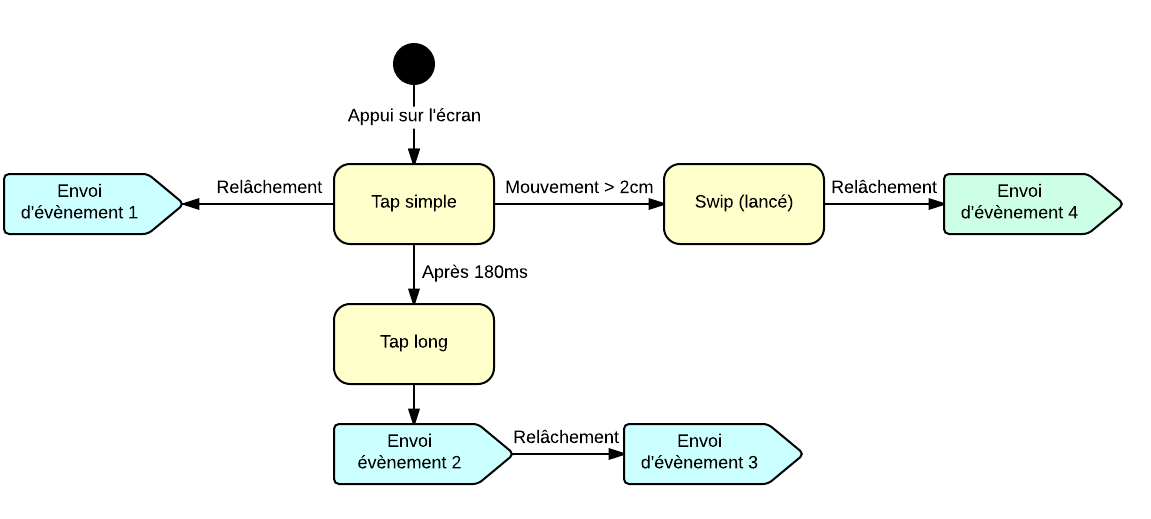
\includegraphics[scale=0.7]{./img/diagEtatTransition.png}
  \caption{Diagramme d'états-transitions des évènements}
  \label{diagetattrans}
\end{figure}


\paragraph{}
La gestion des évènements est délicate, dans le sens où elle se joue à quelques millisecondes prêt. Un temps d'attente trop long, et le joueur retrouve un décalage entre le moment où il appuie, et le moment où l'évènement est envoyé. Trop court, et le tap bref est interprété par un tap long, et le glissé n'a pas le temps de se faire. De même, une distance trop courte, et le moindre mouvement du doigt est interprété comme un lancement. Trop longue, et le risque qu'il soit interprété comme un évènement long, ou qu'un décalage se créé, apparaît. Ainsi de nombreux tests ont dû être effectués, nécessitant un mouvement infime des paramètres, et demandant à chaque fois de faire de nouveau une compilation, un transfert sur le téléphone et un test, puisque seule l'expérimentation permet de savoir si le réglage est bon.

\paragraph{Détection de la réussite}
Une fois les évènements convertis en numéros d'action, il faut vérifier si ces numéros sont en cohésion avec le niveau chargé. On ne compte que les échecs, et à la fin du niveau on soustrait le nombre total d'actions à réaliser par le nombre d'échecs pour obtenir le \% de réussite sur le niveau.
On ne met pas en place d'échelle de réussite comme on peut voir dans les autres jeux (mauvais, bon, parfait...). On considère que le joueur réussit ou rate un évènement.\\\\
Il y a deux types d'évènements à tester :
\begin{itemize}
\item Au moment où le joueur appuie, il faut vérifier que le numéro d'action tapé correspond au numéro d'action courant du niveau. On incrémente le nombre d'échecs si ça ne correspond pas.
\item Quand un évènement est passé, il vérifie si le joueur l'a réussi. Dans le cas où le joueur ne joue pas, il faut compter des erreurs.
\end{itemize}
\paragraph{}

La phase complexe est de déterminer quand un évènement est trop tôt ou trop tard. Un joueur ne frappera jamais pile au moment réel de l'évènement : Il faut mettre en place un système de tolérance.
\\\\
Après de multiples tests, nous avons conclu que le délais d'un quart de temps est suffisant comme négligence. C'est à dire que le joueur dispose d'un quart de temps complet pour réaliser une action demandée.
\\\\
On stocke dans une liste les numéros des ticks où le joueur a réussi. Quand le \textit{beateur} envoie un évènement, on regarde si le joueur a réussi le précédent. Sans quoi, on envoie un évènement \texttt{onFailure}.
\\\\
N'importe quel objet Unity peut se connecter à ce contrôleur. Ceci permet de construire le feedback visuel, en jouant par exemple une animation quand on reçoit un évènement \texttt{onFailure}.

\subsection{Résumé}
\label{engine_summary}
\noindent
\makebox[\textwidth]{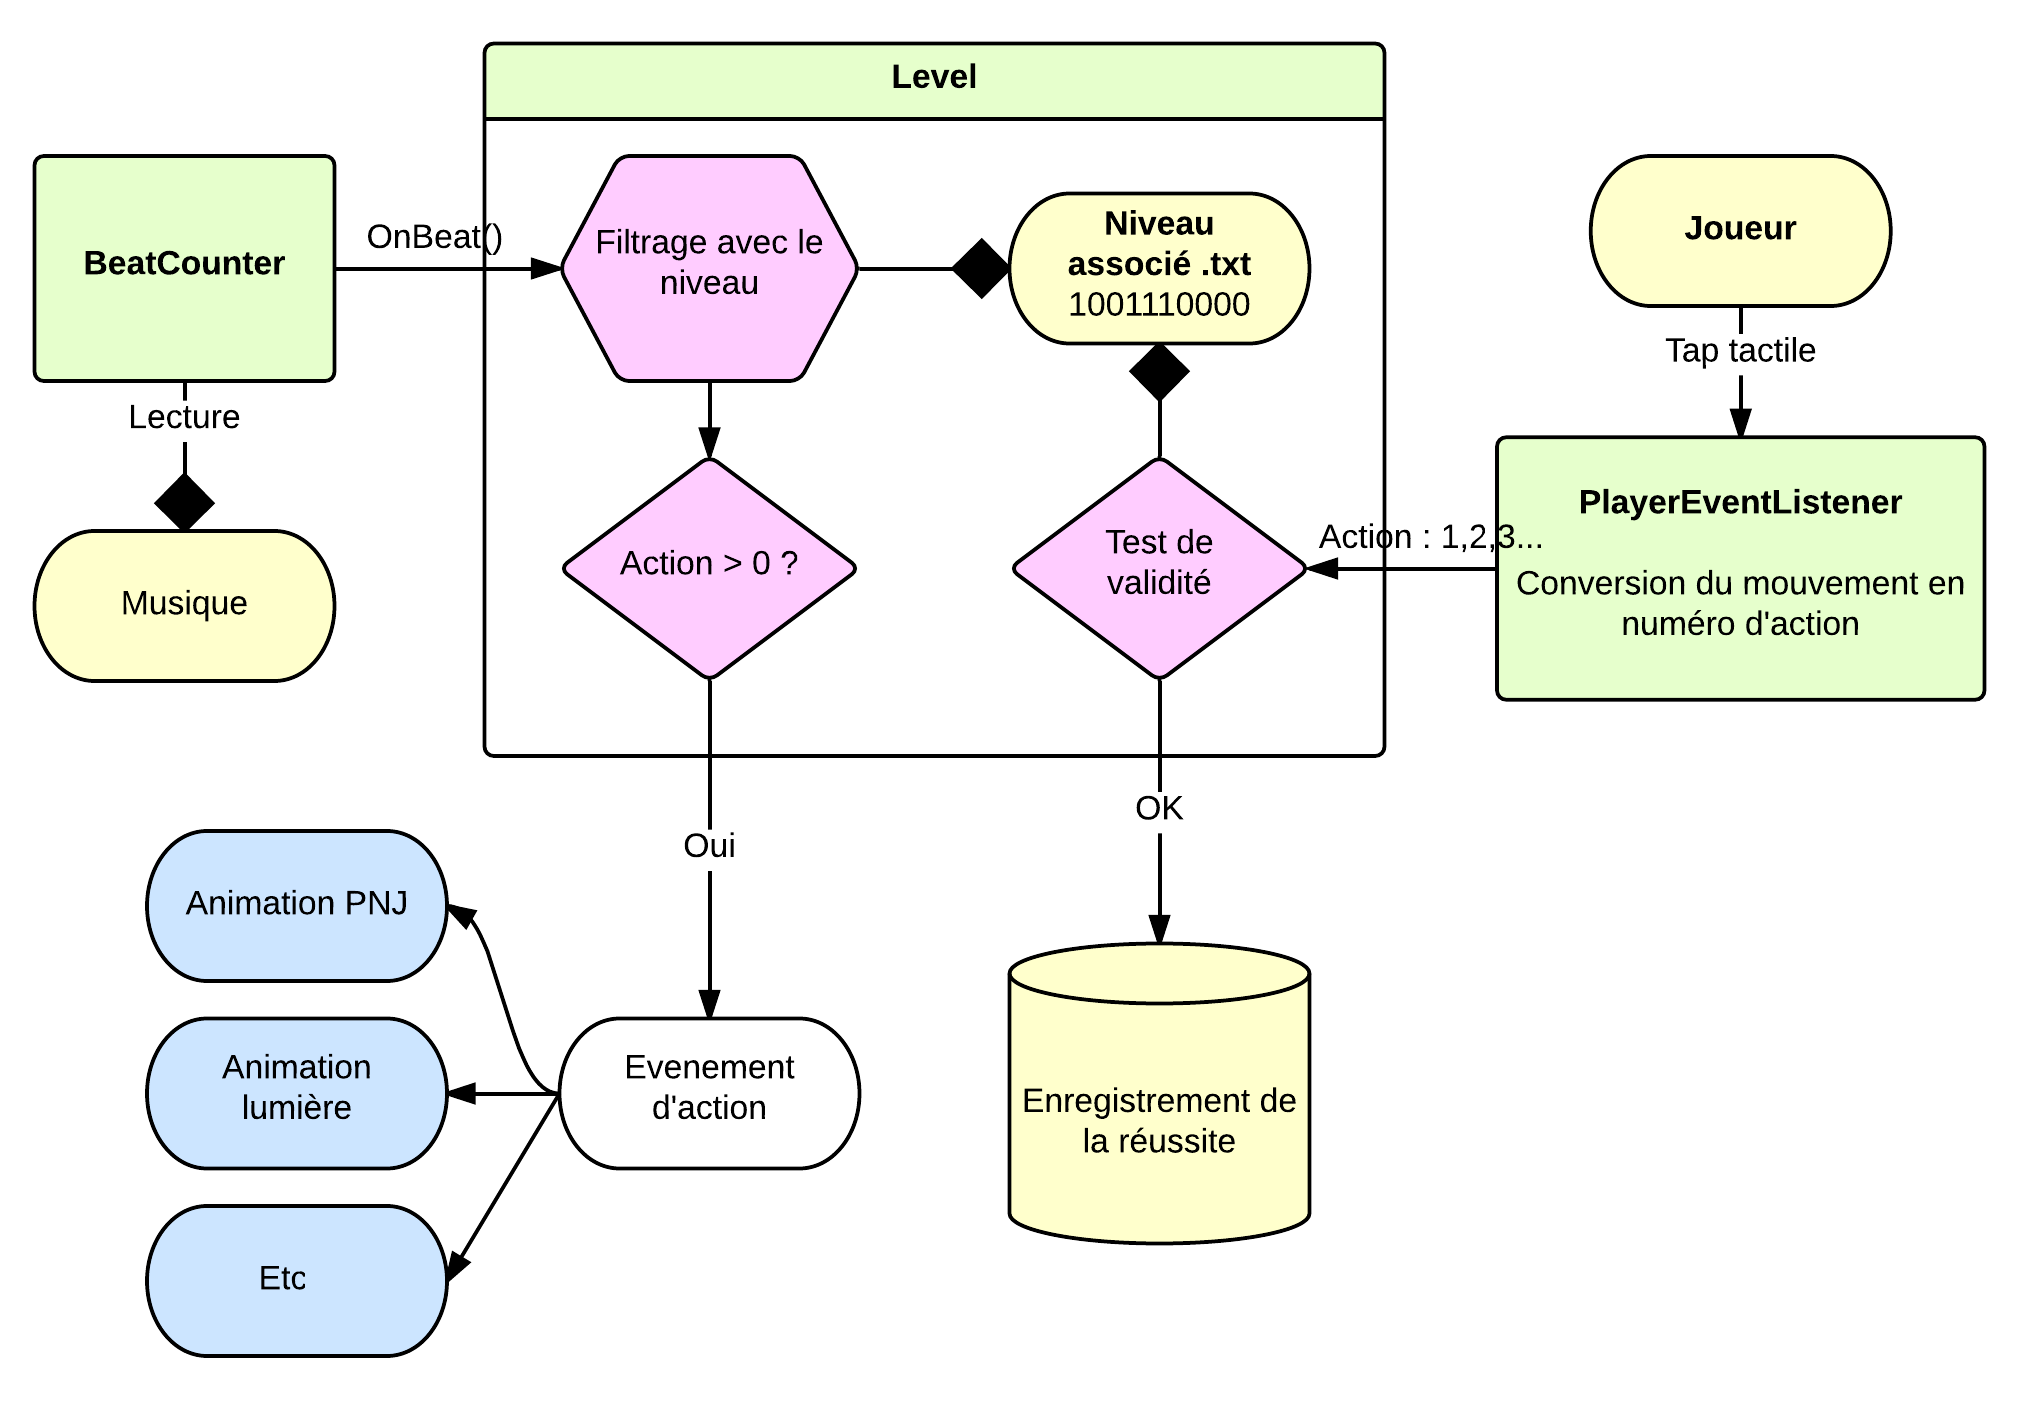
\includegraphics[scale=1]{./img/diagramme_moteur.png}}
\paragraph{}

Pour résumer le fonctionnement du moteur :
\begin{itemize}
\item Le \texttt{BeatCounter} lit la musique et envoie des évènements \texttt{OnBeat()} à chaque quart de temps.
\item Le \texttt{LevelScripted} filtre ces évènements en lisant le fichier, et envoie des évènements d'actions à tout les objets Unity qui l'écoutent
\item Quand le joueur tape sur l'écran, le \texttt{PlayerEventListener} convertit le mouvement en numéro d'action
\item Les actions du joueur sont validées par le \texttt{PlayerActions} qui enregistre si l'action correspond au fichier
\end{itemize}

\section{Outil de construction des niveaux}

Même si notre système de fichier texte est suffisamment clair pour être lu et modifié manuellement, il est tout de même fastidieux de construire des niveaux directement. Il est beaucoup plus intéressant de créer les actions du niveau dans un logiciel de musique. Nous avons donc développé un outil de conversion pour générer un niveau à partir de fichiers MIDI.

\section{Choix du langage}
La programmation est la représentation des données et la manipulation de ces représentations. Les fichiers midi sont représentés par des listes de listes. Quel meilleur langage qu'un LISP pour effectuer des opérations sur des listes ? Le Scheme s'est imposé comme choix naturel.

\subsection{Structure d'un fichier midi}
Les spécifications du midi sont lourdes et complexes, elles ne seront pas détaillées ici, seules seront détaillées les informations importantes à notre convertisseur de niveau.

Un fichier midi est composé d'une suite de "chunks", eux mêmes composés d'évènements, il existe un certain nombre d'évènements différents, tels que le nom de la piste, le tempo, le nombre de pistes... Nous détaillerons uniquement les événements pertinents à notre programme.\\
{\small \texttt{fichier midi = <header chunk> + <track chunk> [+ <track chunk> ...]}}\\\\
Un fichier midi commence par un \textit{header} formé de la manière suivante :\\
{\small \texttt{header chunk = "MThd" + <header length> + <format> + <n> + <division>}}\\

\begin{lstlisting}[style=Scheme]
;; lecture de l en-tete du fichier
(define (read-header in)
    (header (to-string (read-n-bytes in 4))
            (to-int (read-n-bytes in 4))
            (to-int (read-n-bytes in 2))
            (to-int (read-n-bytes in 2))
            (to-int (read-n-bytes in 2))))
\end{lstlisting}
{\small \texttt{track chunk = "MTrk" + <length> + <track event> [+ <track event> ...]}}\\\\
Un \textit{event} se présent sous la forme suivante :\\
{\small \texttt{track event = <delta time> + <midi event> | <meta event>}}\\\\
Les \textit{meta events} servent à donner des informations telles que le tempo, la division du tempo, ou la fin d'une \textit{track}.\\

\begin{lstlisting}[style=Scheme]
;; events utilises
(define time-signature-event '(255 88 4))
(define set-tempo-event '(255 81 3))
(define sequence-name-event '(255 3))
(define instrument-name-event '(255 4))
(define key-signature-event '(255 89 2))
(define smpte-offset-event '(255 84 5))
(define midi-channel-prefix-event '(255 32 1))
(define end-event '(255 47 0))
\end{lstlisting}

Les \textit{midi events} sont quand à eux des évènements directement en rapport avec la musique, le début ou la fin d'une note, ou encore le changement de canal.
{\small \texttt{midi event = <status byte> + <data byte> + <data byte>}}\\\\
Un fichier midi est un fichier binaire, à sa lecture, c'est une suite de valeurs hexadécimales, il est représenté dans notre programme comme une suite de valeurs de 0 à 255 : ‘(20 255 88 4 60 100 ...).

En parcourant le fichier, on peut reconnaître par exemple la suite d'octets "255 88 4", qui fait partie de nos évènement connus, on connaît également la taille de cet évènement, on sait donc que les 4 octets suivants formeront un \textit{event} de type "time signature".\\

\begin{lstlisting}[style=Scheme]
;;vrai si toutes les valeurs de l1 sont dans l2
(define (sublist? l1 l2)
    (andmap (lambda (i j)
        (= i j)) l1 (take l2 (length l1))))

;;vrai si les premiers octets de data
;;forment un event connu : e
(define (known-event? e data)
    (or (sublist? e data) (sublist? e (cdr data))))
\end{lstlisting}

Le delta time est codé avec une quantité à longueur variable. Le delta time n'est pas par rapport au début de la piste mais par rapport à l'évènement précédent. C'est lui qui permettra à la musique dans le fichier midi d'avoir un rythme, par exemple, plus le delta time est long entre un évènement de début de note et un évènement de fin de note, plus la note sera tenue longtemps.\\\\

\fbox{\parbox{11cm}
{\textbf{Note technique sur la quantité à longueur variable (\textit{variable-length quantity})}\\La vlq permet de représenter de manière compacte des quantités supérieures à un octet.

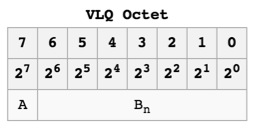
\includegraphics[scale=1]{./img/vlqOctet.png}\\
Si \texttt{A} est égal à 0, c'est que c'est le dernier octet de la quantité. Si c'est 1, un autre octet vlq suit.\\
\texttt{B} est un nombre de 7 bits, et \texttt{n} est la position de l'octet où \texttt{B0} est l’octet de poids faible.}
}\\\\

Certains éditeurs de fichiers midi utilisent une technique appelée le "running status" pour réduire la taille de leurs fichiers. Pour clairement comprendre son fonctionnement, une explication supplémentaire sur les \textit{midi events} s'impose.

Le \textit{status byte} a une valeur comprise entre 128 et 255, les \textit{data bytes} ont, quant à eux, une valeur comprise entre 0 et 127.

Le "running status" consiste à ne pas répéter le \textit{status byte} s'il est identique à l'évènement précédent. L'utilisation du "running status" est triviale à détecter et implémenter. En lisant le fichier, si l'octet lu est inférieur à 128 alors que l'on attendait un \textit{status byte}, c'est qu'il faut utiliser le dernier \textit{status byte} rencontré.

\subsection{Conversion en niveau}

En possession des ces informations, et avec la table des codes midi (voir annexe), convertir le fichier midi en niveau n'est alors plus qu'une succession de transformation de représentations. D'abord en \textit{chunks}, puis en \textit{tracks}, et enfin en \textit{events}, en filtrant les évènements inutiles à notre cas d'utilisation.\\
Une fois les évènements extraits du fichier midi, nous sommes en mesure de les convertir en actions pour notre jeu.

L'action 1 correspond à la note C, l'action 2 à la note C\#, et l'action 3 à la note D.
À chaque évènement avec le \textit{status byte} "début de note" (de l'octet 0x90 à l'octet 0x9F), l'action correspondant à la note de l'évènement est ajoutée au niveau. Ces actions sont séparées avec des zéros, eux donnés par le \textit{delta time}.\\

\begin{lstlisting}[style=Scheme]
;; transforme un evenement en donnees de niveau (0, 1, 2...)
;; division est le nombre de frames par secondes
;; delta-sum est la somme des delta depuis le dernier event utile
(define (event-to-level event division delta-sum)
    (let ([n (/ (+ delta-sum (vlq->int (midi-event-delta event))) (/ division 4))])
         ; n est le nombre de temps ou rien ne se passe (0)
         ; midi-event-arg1 est la note
         ; notes est la hashmap ou sont faites les correspondances
         (append (make-list n 0) `(,(hash-ref notes (midi-event-arg1 event) ?)))))
\end{lstlisting}


\subsection{Mise en pratique}
On utilise dans cet exemple le logiciel Logic Pro X sous Mac OS X. N'importe quel autre séquenceur gérant les fichiers MIDI peut être utilisé.\\

\paragraph{}
On importe la musique sur une piste, et on indique au logiciel son tempo (qui doit être connu, on peut utiliser un logiciel commit \textit{Audacity} pour le détecter).

\begin{figure}[H]\centering
  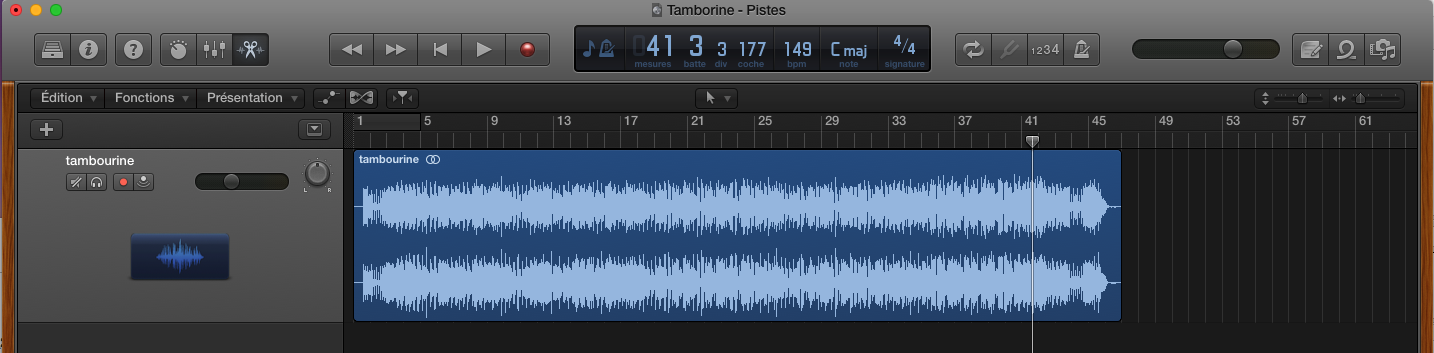
\includegraphics[width=11cm]{./img/logic_sound.png}
  \caption{Piste sonore}
  \label{transitions_scenes}
\end{figure}

\paragraph{}
On ajoute sur une seconde piste vide un instrument qui représente le niveau à créer, sur laquelle on va ajouter les actions.\\

\begin{figure}[H]\centering
  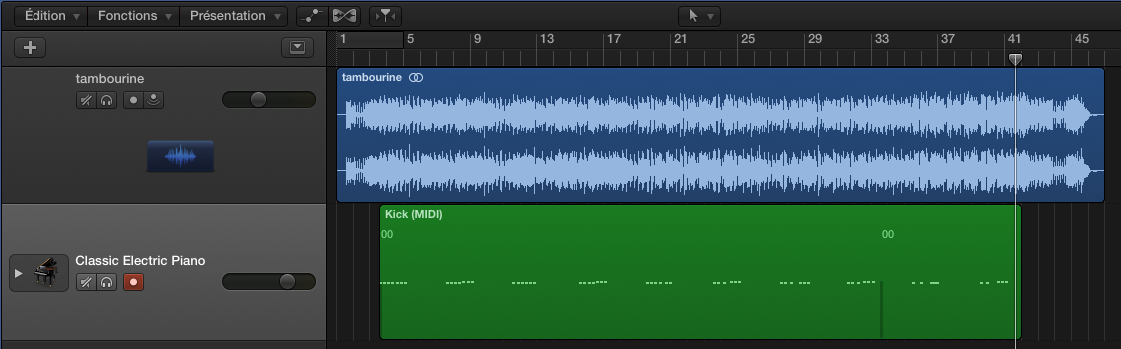
\includegraphics[width=11cm]{./img/logic_midi.png}
  \caption{Piste MIDI}
  \label{transitions_scenes}
\end{figure}


\paragraph{}
On pose ensuite les notes qui représentent les actions sur cette piste, puis on écoute le tout en temps réel pour superposer proprement chacune des actions sur la musique. On utilise des notes différentes pour chaque type d'action. Ici le DO pour une action 1, le DO\# pour une action 2, etc.

\begin{figure}[H]\centering
  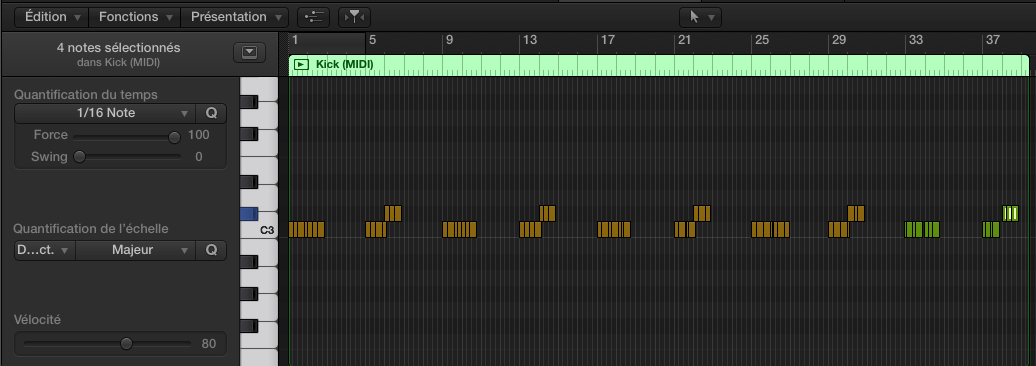
\includegraphics[width=11cm]{./img/logic_edit.png}
  \caption{Éditeur de notes de Logic Pro}
  \label{pianoroll}
\end{figure}

\paragraph{}
Une fois le niveau construit, il ne reste plus qu'à exporter la piste au format .midi, et de le passer au convertisseur pour obtenir le niveau au format .txt.

\begin{figure}[H]\centering
  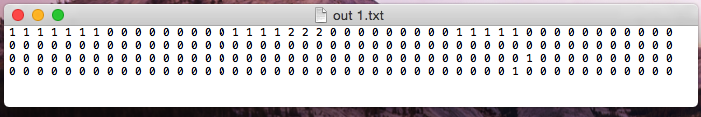
\includegraphics[width=11cm]{./img/logic_export.png}
  \caption{Fichier .txt du niveau en sortie}
  \label{level}
\end{figure}

\section{Avancement du joueur}

\subsection{Calcul du score dans un mini-jeu}

Le calcul du score est fait sous la forme d'un pourcentage. En fait, seul le nombre d'erreur est regardé, puisque peu importe que le joueur fasse tout bon, si il se contente d'envoyer des évènements dans tous les sens en appuyant sur son tactile. C'est pourquoi le nombre de réussite n'est pas regardé à proprement parler. Cependant est considéré comme un échec:
\begin{itemize}
\item Un évènement envoyé à un moment non attendu
\item Un évènement envoyé alors que c'est un autre qui est attendu
\item Ne pas envoyer d'évènement alors qu'un évènement est attendu
\end{itemize}
Ainsi, même si les succès ne sont pas considérés, étant donné que l'absence de succès est considérée comme un échec, ne rien faire ou spammer le tactile ne donne en aucun cas un bon score, pas moyen de “tricher” pour gagner, la seule manière étant de jouer correctement.
Ensuite, une fois les échecs additionnés, on se contente de calculer le pourcentage en divisant le nombre d'échec par le nombre d'évènement attendu. Ainsi, 0 correspond au fait de n'avoir fait aucun échec, 1 correspond au fait d'avoir fait autant d'échec que d'étapes à effectuer (plus voulant dire qu'on a fait plus d'erreurs que d'étapes). On soustrait ce nombre à 1, et on multiplie par 100 pour obtenir un pourcentage. On se retrouve donc à avoir 100\% si on n'a fait aucune erreur, 50\% si on a loupé la moitié des évènements, et on renvoie 0\% si on fait autant d'erreurs ou plus que d'évènements à faire. 

\subsection{Enregistrement des scores}

Même si le calcul des scores est fait sous la forme de pourcentage, ce qui est affiché au joueur et ce qui est enregistré est sous la forme d'étoiles. 3 étoiles correspond à 100\% de réussite, 2 étoiles à un score supérieur à 90\% et enfin 1 étoile à un score supérieur à 75\%. Le score est enregistré de manière très simple, Unity permettant d'enregistrer des entiers, des chaînes de caractères et des nombres flottants. Ainsi le score est enregistré dans une variable "int" s'appelant “etoileLevel[numéro du mini jeu]” et sa valeur correspond au nombre d'étoiles. A chaque fin d'un mini-jeu, on vérifie si le joueur n'a pas amélioré le nombre d'étoiles sur ce mini-jeu, et si oui, alors on écrase le précédent score avec le nouveau qui est meilleur.

\begin{figure}[H]\centering
  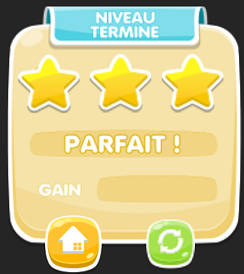
\includegraphics[scale=.9]{./img/MenuMort.png}
  \caption{Score du joueur affiché}
  \label{SelectionMiniJeu}
\end{figure}

\subsection{Déblocage des mini-jeux}

Certains jeux sont débloqués de base, d'autres nécessitent la réussite d'un autre mini-jeu pour cela. Un mini-jeu est considéré comme réussi du moment que le joueur a obtenu au moins une étoile sur ce jeu. Ainsi, si un mini-jeu n'est pas débloqué, dans le menu de sélection des mini-jeux, son icône est grisée, et il est inclicable. De plus, en dessous de l'icône de chaque mini-jeu est affiché le plus grand nombre d'étoiles obtenu dans le jeu correspondant.

\begin{figure}[H]\centering
  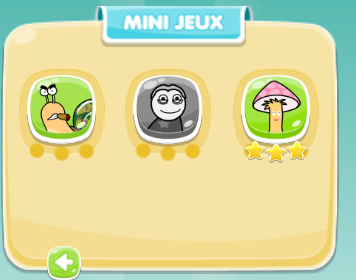
\includegraphics[scale=.9]{./img/SelectionMiniJeu.png}
  \caption{Sélection des mini-jeux}
  \label{SelectionMiniJeu}
\end{figure}

\section{Création d'un mini-jeu}

Afin d'obtenir un niveau cohérent, le processus de création d'un mini-jeu doit se faire étape par étape. Le travail effectué sur le premier niveau a permis de peaufiner ce processus et de réaliser les mini-jeux suivants avec plus d'efficacité et de rapidité. Dans un premier temps, nous avons commencé à développer le niveau des champignons en suivant des étapes qui nous paraissaient logiques. Puis, après avoir développé la majeure partie du niveau, nous avons réalisé qu'il manquait des éléments importants au gameplay, tels que des sons cohérents correspondants au rythme et à l'image, ou un \textit{feedback} visuel montrant la réussite ou l'échec du joueur.

Pour illustrer ces différentes étapes, des exemples seront tirés du mini-jeu des champignons.

\subsection{Les graphismes}

Un des éléments les plus importants d'un jeu est son aspect visuel. Il est préférable de commencer par avoir une base solide au niveau de ce que l'on veut que le joueur fasse. Ensuite, il s'agit d'imaginer une scène simple dans laquelle l'action du joueur ne serait pas aberrante. Par exemple, si le joueur doit répéter un motif sonore, alors il vaut mieux que les graphismes représentent au moins deux personnages frappant sur une surface, un représentant le modèle, et l'autre le joueur.

Dans notre projet, nous avons voulu mettre en avant le côté simple et divertissant de notre thème en utilisant des graphismes 2D de type \textit{cartoon}. Nous avons créé nos propres graphismes, en utilisant des couleurs vives et des traits de contours très épais.

\begin{figure}[H]\centering
  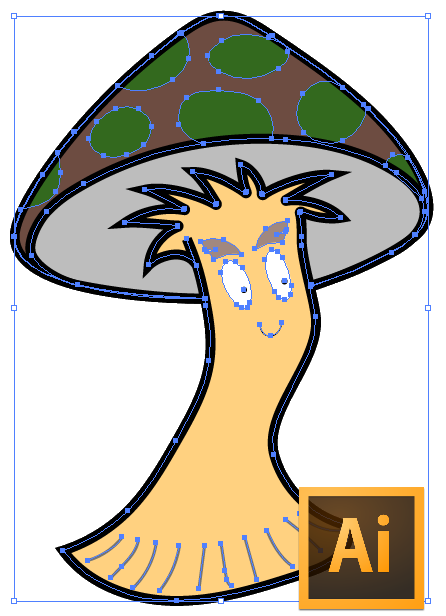
\includegraphics[scale=.6]{./img/technique_graphismes.png}
  \caption{Exemple visuel de fichier graphique vectoriel}
  \label{SelectionMiniJeu}
\end{figure}

Pour cela nous avons utilisé Adobe Illustrator, qui permet de réaliser des créations graphiques vectorielles. L'intérêt de travailler sur du vectoriel est qu'on peut rendre l'image dans la dimension voulue, et, de plus, il est plus facile d'apporter rapidement une petite modification un objet ou sa couleur, sans avoir tout à recommencer.

\subsection{Les animations}
\label{anims}
Les animations utilisées dans l'application sont gérées directement par Unity. Leur mise en place est classique, elle se fait via l'utilisation de clés sur une ligne de temps. 

\begin{figure}[H]\centering
  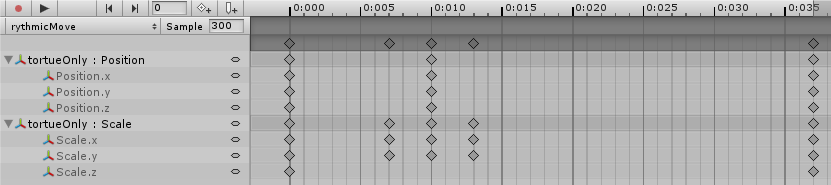
\includegraphics[scale=.55]{./img/technique_animation1.png}
  \caption{Exemple d'utilisation de clés sur une ligne temporelle}
  \label{technique_animation1}
\end{figure}

Le principe étant de donner les caractéristiques de l'objet à animer (position, taille, rotation ...) à un temps donné, et de les stocker dans une clé. Une fois que deux clés ont étés crées, une interpolation linéaire est ensuite appliquée entre les deux clés afin d'obtenir un déplacement fluide sur les images intermédiaires. La courbe d'interpolation peut être modifiée afin d'obtenir l'effet voulu.

\begin{figure}[H]\centering
  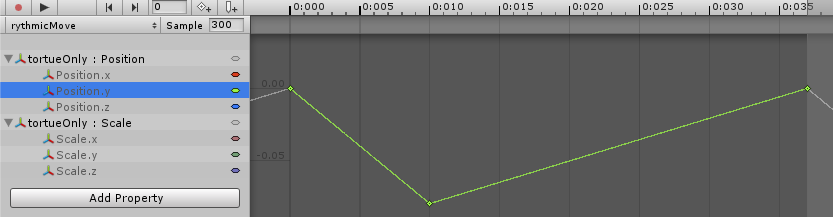
\includegraphics[scale=.55]{./img/technique_animation2.png}
  \caption{Interpolation simple entre trois clés définissant la position y de l'objet}
  \label{technique_animation2}
\end{figure}

Unity possède la caractéristique de pouvoir créer un diagramme d'état afin de jouer les différentes animations dans l'ordre désiré. Dans notre projet, nous avons utilisé cette fonctionnalité pour nous aligner sur le rythme de la musique. Pour cela, nous avons créé un arbre simple qui possède un état \textit{immobile} et un état \textit{mouvement}. A chaque fin d'une animation, c'est l'animation suivante qui sera jouée, en synchronisation avec les battements par minute de la musique.

\begin{figure}[H]\centering
  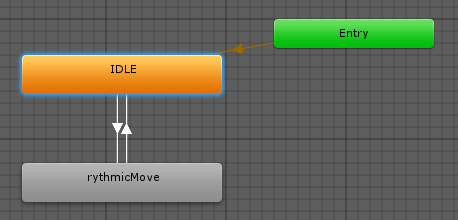
\includegraphics[scale=.55]{./img/technique_animation3.png}
  \caption{Diagramme d'état utilisé pour l'animation}
  \label{technique_animation3}
\end{figure}

\subsection{Assemblage avec le moteur}
On va donc brancher les différents éléments composants le jeu au moteur. Les différents éléments du moteurs sont détaillés partie \ref{engine_summary}.

\paragraph{}
Commençons par les éléments du décor et les personnages non-joueur. Ils seront reliés à un \textit{LevelScripted} auquel on passera en paramètre le fichier texte correspondant à leur mouvement. Les mouvements sont et les animations (voir partie \ref{anims}) déclenchés à l'aide de \textit{trigger} que le \textit{LevelScripted} va envoyer en fonction des évènements lus. \\
Typiquement on aura un \textit{LevelScripted} avec un fichier texte ressemblant à celui fig. \ref{simple_level} qui servira à battre la mesure et à indiquer le tempo au joueur.\\
On aura ensuite un \textit{LevelScripted} avec un vrai niveau qui va scripter les mouvements d'un personnage non-joueur comme on peut le voir par exemple dans le niveau des champignons où le joueur doit répéter les mouvements du PNJ.\\
Les \textit{LevelScripted} sont évidemment reliés au \textit{BeatCounter} pour que tous les mouvements du décor et des PNJ soient effectués en rythme.

\paragraph{}
Les animations du personnage joueur fonctionnent globalement de la même manière. La seul différence est que l'on va ajouter un \textit{PlayerActions} et un \textit{PlayerEventListener} qui vont se charger de récupérer les actions du joueur et d'interroger le \textit{LevelScripted} pour savoir si l'action du joueur correspond à l'action attendue, et ainsi envoyer le trigger correspondant. 

\subsection{Le \textit{feedback}}

Le \textit{feedback} est l'ensemble des signes visuels ou sonores que recevra le joueur en fonction de son action. Dans notre application, il permet de signaler la réussite ou l'échec d'une action de l'utilisateur. Ainsi un coup réussi jouera un son cohérent avec la scène et une animation gratifiante sera jouée, afin de récompenser rapidement le joueur. A l'inverse, une action ratée résultera à un son lié à un échec et des graphismes montrant le mécontentement.
Le feedback retourné par l'application s'est avéré être un des points les plus difficiles à imaginer dans la création des scénarios des mini-jeux.

\subsection{Le choix des sons}

Maintenant que la plupart des éléments sont placés et fonctionnels dans la scène, il s'agit d'ajouter le plus important : la musique. Son rôle est important car c'est sur son rythme que l'utilisateur devra se synchroniser pour réussir le niveau. Elle se doit donc de comporter des rythmes prononcés et un thème en rapport avec la scène créée.
Ne pouvant nous même pas composer notre propre musique, nous avons fait le choix d'ajouter dans notre jeu des musique proposées gratuitement et libres de droit sur Internet.

\subsection{La difficulté}

Après avoir développé tout le contenu d'un mini-jeu, il faut évaluer sa difficulté en se mettant dans la peau d'un joueur qui le découvre pour la première fois. Celle-ci ne doit être ni trop élevée, pour ne pas se décourager, ni trop simple, pour ne pas s'ennuyer. Pour répondre à ce problème, nous avons d'abord placé des motifs simple à réaliser, puis augmenté peu à peu leur difficulté au fur et à mesure de l'avancement du niveau. Ensuite, nous avons fait tester nos ébauches de niveau à des personnes externe au développement qui ont pu juger de la difficulté du jeu.


\section{Les tutoriels}

\paragraph{}
Le tutoriel est crucial dans la perception que le joueur a du jeu, c'est sa première interaction avec le gameplay, la plus importante, celle qui dictera si le joueur restera ou sera rebuté par un gameplay désagréable, inintéressant ou trop difficile. Un tutoriel se doit donc d'être ludique et accessible, tout en enseignant correctement les bases du jeu.

\paragraph{}
Nos tutoriels placent de plus le joueur dans le contexte du jeu, en lui donnant un semblant d'histoire. Le tutoriel est donc divisé en étapes successives, du texte, pour l'histoire et les explications, et une phase de jeu, dans laquelle le joueur applique ce qu'il vient d'apprendre dans la phase précédente. Cette boucle se répète autant de fois qu'il y a de notions à apprendre pour le jeu.

\paragraph{}
Comme expliqué section \ref{niveau}, les niveaux sont scriptés par des fichiers textes. La même technique est utilisée pour les tutoriels, qui ne sont rien d'autres que des niveaux normaux, un fichier texte par étape. À la première étape, le joueur apprendra par exemple le tap court, le fichier texte sera donc uniquement composé de ces évènements, puis lorsque cet élément sera appris, le moteur chargera un autre fichier texte contenant un autre élément de gameplay jusqu'à ce que le joueur les ai tous appris.

\paragraph{}
Pour être certain que le joueur maîtrise un élément de gameplay, et ainsi pouvoir passé à l'étape suivante du tutoriel, il lui est demandé de le répéter trois fois. C'est pour s'assurer que le joueur n'a pas réussi par chance et est donc incapable de completer un niveau, ce qui pourrait entraîner de la frustration.


\begin{figure}[H]\centering
  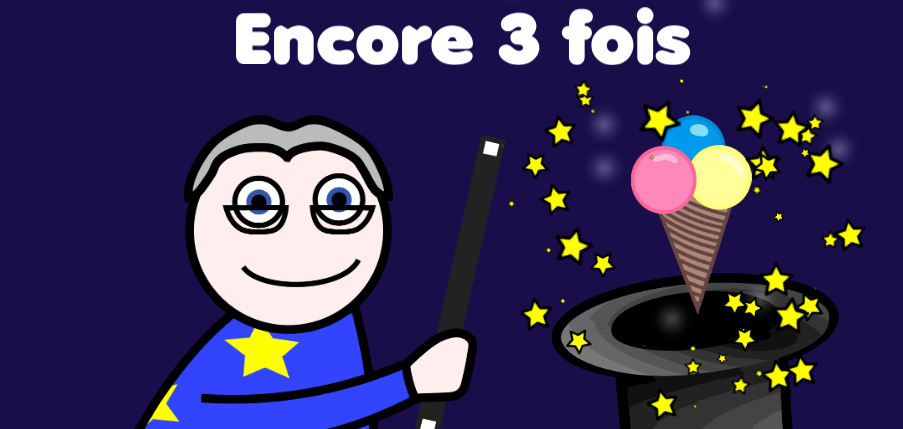
\includegraphics[scale=0.28]{./img/compteur_tuto.png}
  \caption{Compteur du nombre de répétitions restantes}
  \label{repetitions}
\end{figure}

\paragraph{}
Nous avons fait le choix de proposer le tutoriel à chaque fois que le niveau est lancé, désagrément minime pour un joueur expérimenté, mais obligatoire pour un jeu destiné à être partagé et montré. Désagrément minime, mais seulement s'il est possible de passer le tutoriel. Il est donc donné au joueur la possibilité de passer le tutoriel après qu'il l'ai complété au moins une fois.

\begin{figure}[H]\centering
   \begin{minipage}{0.49\textwidth}\centering
     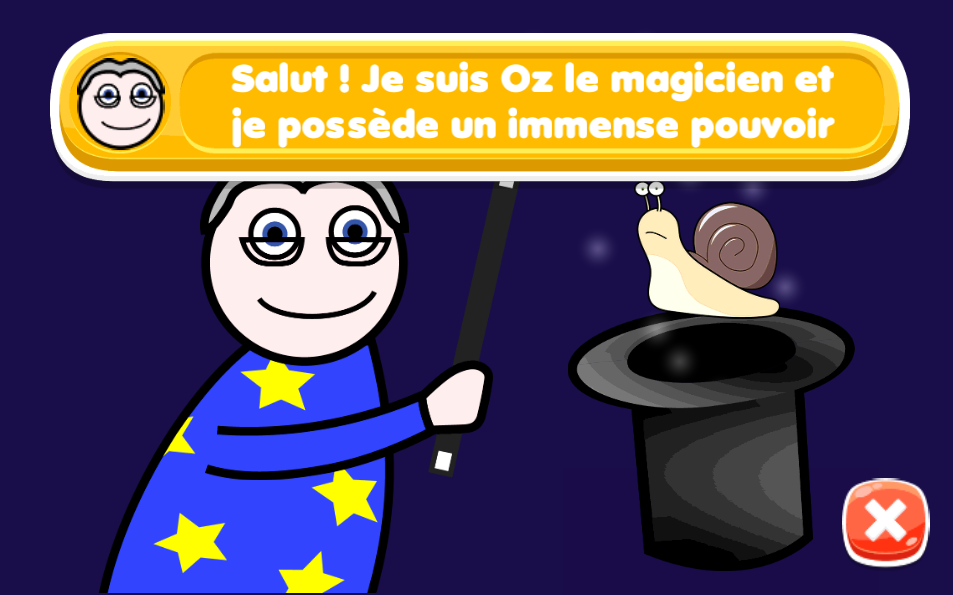
\includegraphics[scale=0.2]{./img/skip_locked.png}
     \caption{Bouton skip verrouillé}
     \label{skip_locked}
   \end{minipage}
   \begin {minipage}{0.49\textwidth}\centering
     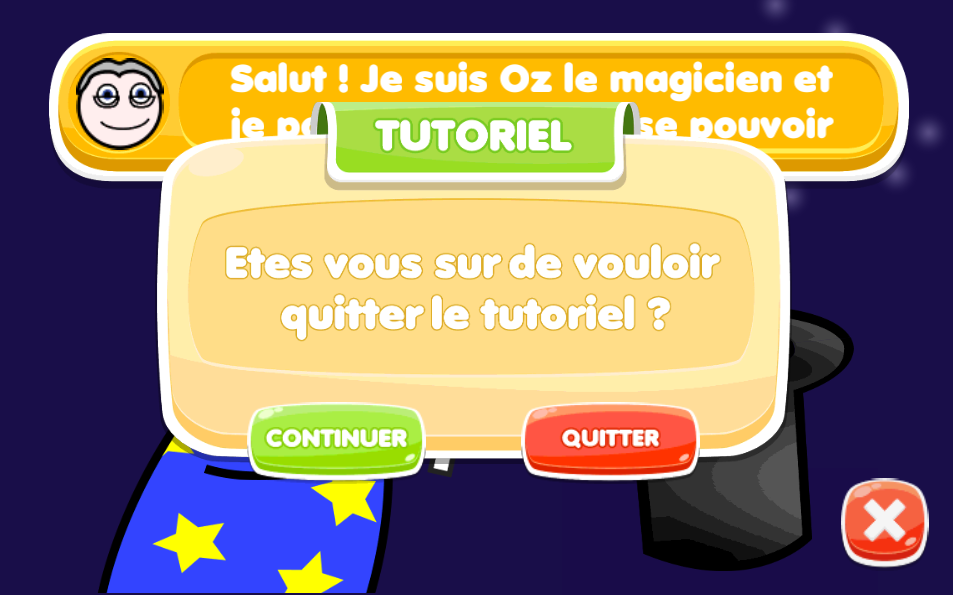
\includegraphics[scale=0.2]{./img/skip_locked_popup.png}
     \caption{Pop up correspondante}
     \label{skip_locked_popup}
   \end{minipage}

 \begin{minipage}{0.49\textwidth}\centering
     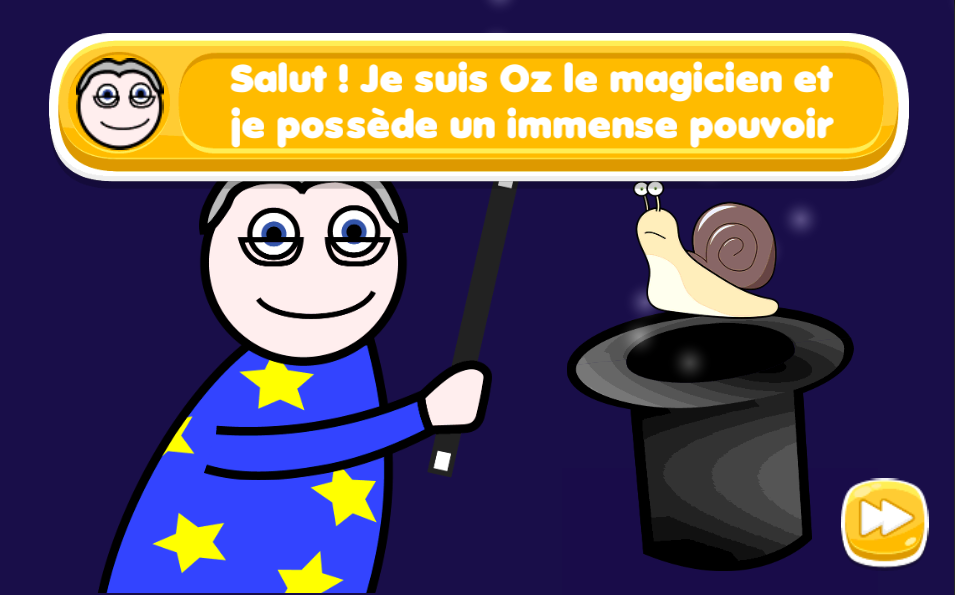
\includegraphics[scale=0.2]{./img/skip_unlocked.png}
     \caption{Bouton skip déverrouillé}
     \label{skip_unlocked}
   \end{minipage}
   \begin {minipage}{0.49\textwidth}\centering
     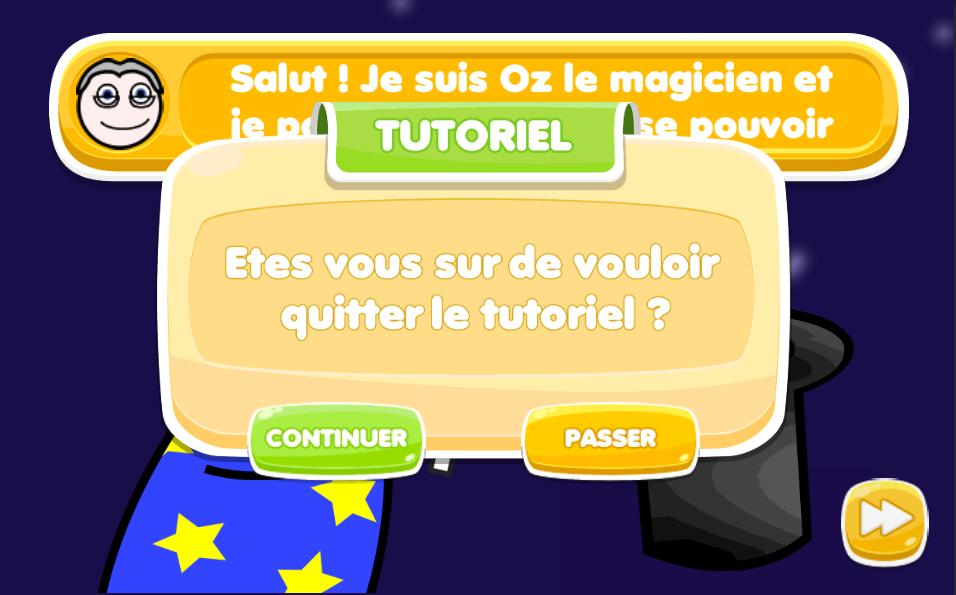
\includegraphics[scale=0.2]{./img/skip_unlocked_popup.png}
     \caption{Pop up correspondante}
     \label{skip_unlocked_popup}
   \end{minipage}
\end{figure}

\paragraph{}
En pratique, un tutoriel est composé d'un tableau de \textit{StepTuto}, chaque \textit{StepTuto} correspond à un élément du tutoriel : un texte ou une phase de jeu. Chaque classe implémentant \textit{StepTuto} possède une méthode \textit{endStep()} qui permettra au tutoriel de passer à l'étape suivante. Cette méthode est appelé lorsqu'un step est terminé, c'est à dire que le joueur a touché l'écran après avoir lu le texte ou qu'une phase de jeu a été réussie. Lorsque toutes les éléments du tableau ont été visités, c'est à dire que toutes les étapes du tutoriel sont achevées, le tutoriel est terminé.

\section{Assemblage des jeux}
\paragraph{}
Chaque jeu est en réalité une scène de Unity. La navigation entre les scènes se fait suivant le diagramme fig. \ref{transitions_scenes}. L'écran principal est un ``hub'' où sont regroupés tous les jeux, on accède bien évidemment au jeu en cliquant dessus. Le tutoriel est ensuite chargé, puis enfin le jeu, on peut remarquer que l'on peut à tout moment revenir à l'écran principal.

\begin{figure}[H]\centering
  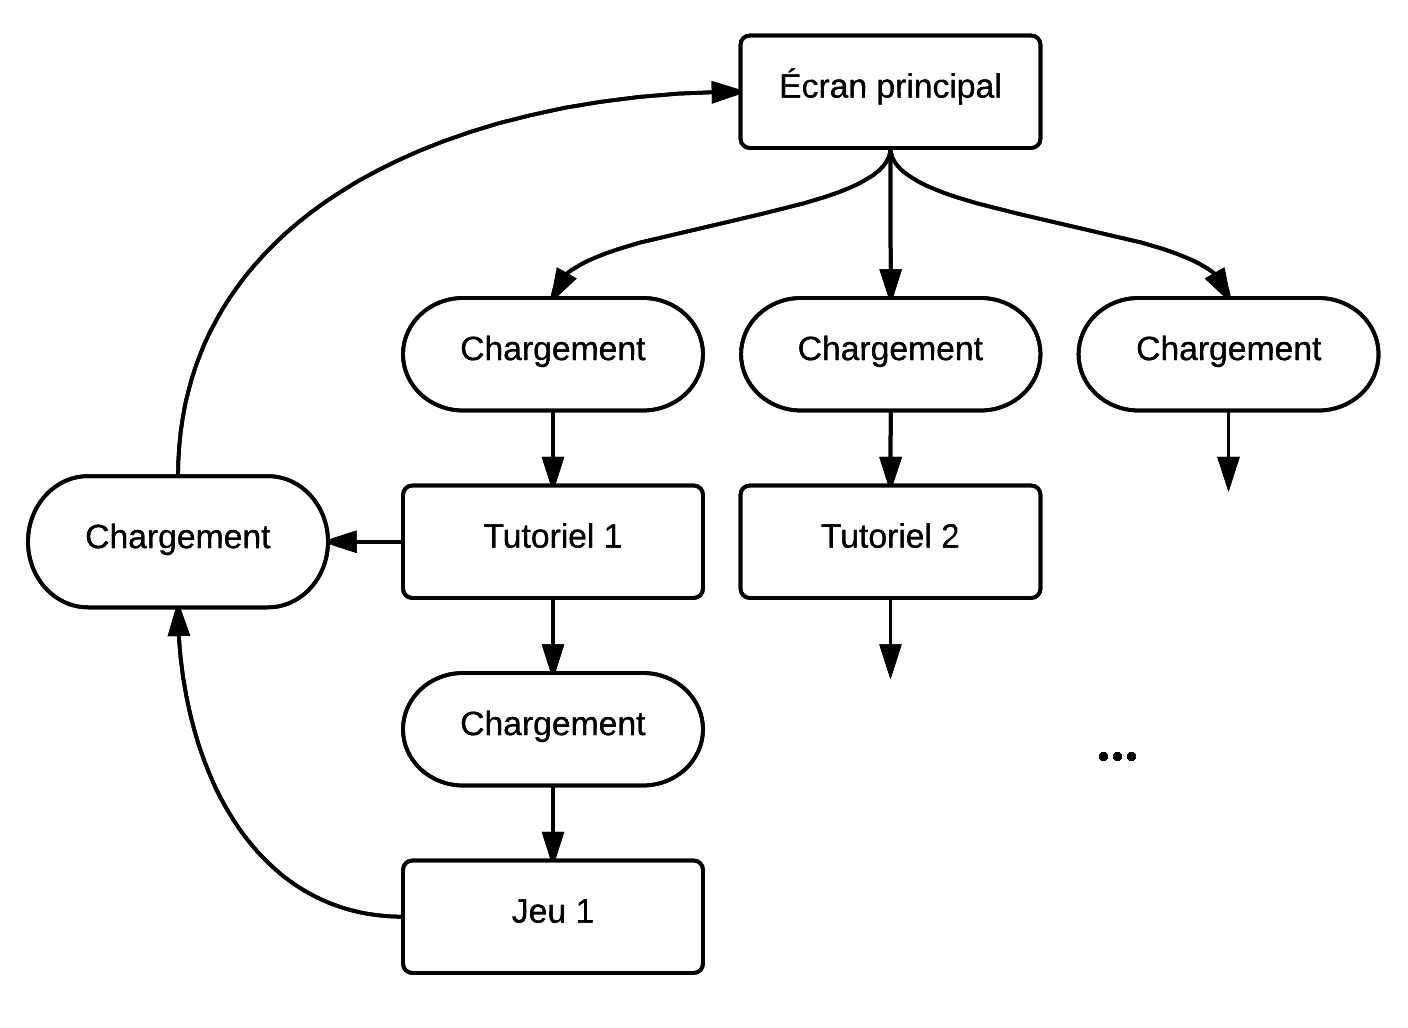
\includegraphics[scale=0.7]{./img/scenes-transitions.png}
  \caption{Transitions entre les scènes du jeu}
  \label{transitions_scenes}
\end{figure}

\paragraph{}
Les scènes ne se chargent pas instantanément, en Unity indique le pourcentage de la scène qui a été chargé, cela permet entre autre de réaliser des écrans de chargement animés. En plus de donner au joueur l'avancement du chargement, cela rend le jeu bien plus fluide que si le chargement était simplement un écran noir, comportement par défaut de Unity.

\begin{figure}[H]\centering
  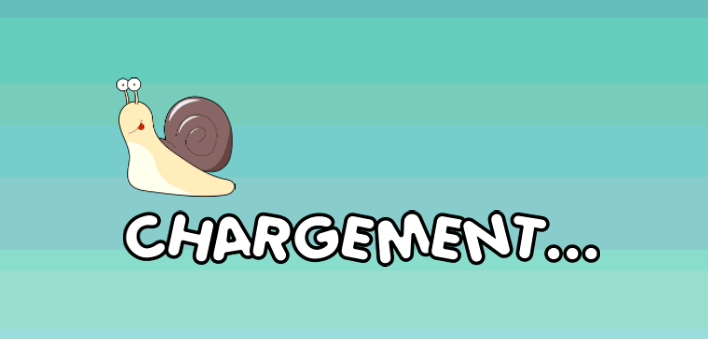
\includegraphics[scale=0.3]{./img/loading.png}
  \caption{Écran de chargement}
  \label{loading}
\end{figure}

\paragraph{}
Les transitions entre les scènes se font donc par des écrans de chargements, mais il serait un peu brusque d'interrompre directement le jeu lorsqu'il est terminé. Nous avons décidé de faire une fermeture en cercle (voir fig. \ref{cartoon}) sur un élément de la scène pour donner un effet cartoon.

\begin{figure}[H]\centering
   \begin{minipage}{0.49\textwidth}\centering
     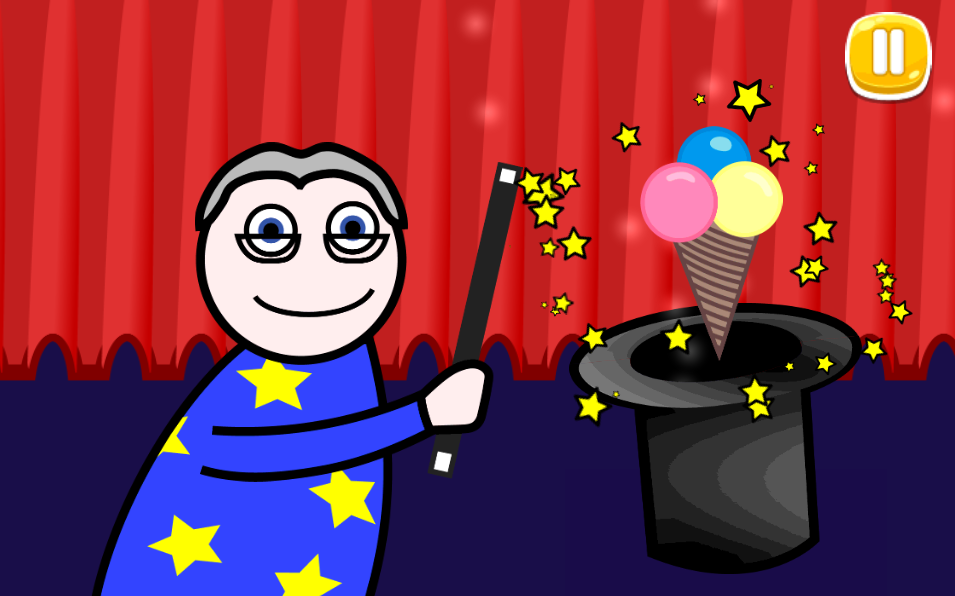
\includegraphics[scale=0.2]{./img/scene.png}
     \caption{Scène normale}
     \label{regular_scene}
   \end{minipage}
   \begin {minipage}{0.49\textwidth}\centering
     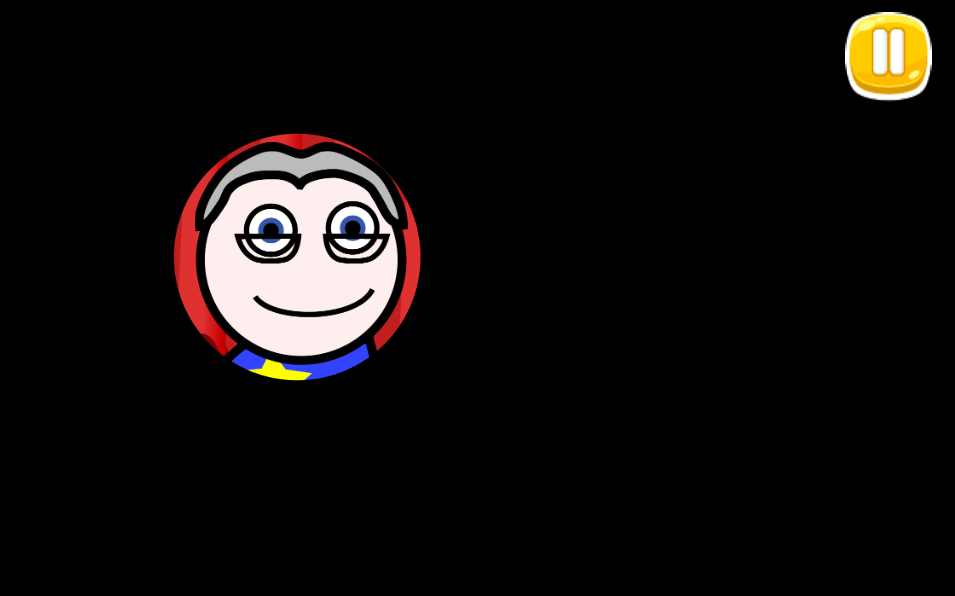
\includegraphics[scale=0.2]{./img/cartoon.png}
     \caption{Fermeture en cercle}
     \label{cartoon}
   \end{minipage}
\end{figure}

Il faut savoir qu'il n'y a pas de manière simple de réaliser cet effet dans Unity. L'approche logique aurait été de coller de grandes zones noires aux bords de l'image du cercle vide, mais il n'est pas possible de manipuler la position et la taille des éléments dans Unity, ces données sont modifiée par le \textit{scale} (échelle) de l'image. Difficile donc d'avoir un effet précis et fluide en multipliant la taille de l'image par un scalaire. C'est la solution de la physique qui a finalement été choisie, un centre de gravité au centre du cercle, et en soumettant les grandes zones noires à la physique, elle se déplacent de façon fluide en suivant le bord du cercle, qui lui a son scale diminué.

\section{Services externes}
Outre le jeu à proprement parler, nous avons intégré d'autres services externes afin de monétiser notre jeu, et d'obtenir des statistiques intéressantes.

\subsection{Statistique et Analyse}

\paragraph{}
La première priorité étant de pouvoir par la suite améliorer le jeu, et pour ce faire, nous avions besoin de savoir comment les utilisateurs interagissent avec notre application. Il se trouve que Google fourni une très bonne interface pour fournir des statistiques d'utilisation: “Google Analytics”. Et un pluggin permettant d'utiliser ces services avec Unity existe. "Google Analytics" est un service qui permet d'analyser le comportement des utilisateurs sur les applications. 

\paragraph{}Il fournit différents outils, qui permettent de connaître la zone géographique de nos utilisateurs, le matériel utilisé, la durée moyenne d'utilisation de notre application, la manière dont ils ont trouvé l'application, mais aussi leurs habitudes d'utilisation, les écrans qu'ils visitent, leur passage ou non des tutos et pleins d'autres informations utiles. Bien utilisé, il permet donc de connaître vraiment le rapport qu'entretiennent les joueurs avec le jeu, et ainsi de donner des pistes sur les améliorations possibles, tant en terme de marketing que sur le jeu lui même. En gros, un outil indispensable pour qui souhaite améliorer son produit, et augmenter le nombre de téléchargements.

\begin{figure}[H]\centering
  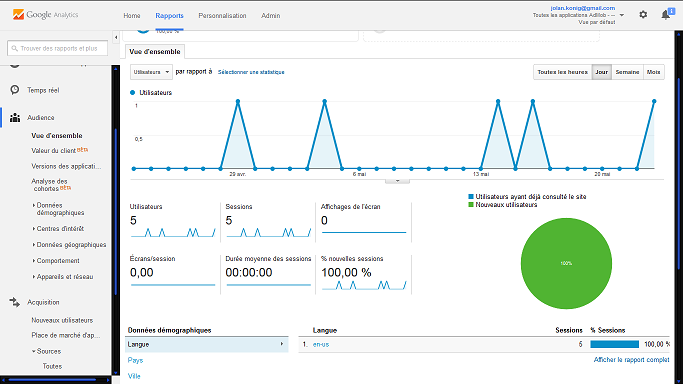
\includegraphics[scale=0.7]{./img/GoogleAnalytics.png}
  \caption{Aperçu des statistiques fournies pas Google Analytics}
  \label{analytics}
\end{figure}

\subsection{Publicité}

\paragraph{}Ensuite, la monétisation à proprement parler. Nous avons opté pour un jeu gratuit, sans boutique, mais monétisé à partir de la publicité. Sur le support mobile, 3 grandes régies publicitaires dominent, Admob (Google), Iad (Apple) et Chartboost. Nous avons choisis Chartboost, pour plusieurs raisons. La première étant qu'elle est réservée pour les jeux mobiles, ainsi nous étions sûr d'avoir des publicités ciblées, et adaptées à nos utilisateurs. Ensuite leur système de rémunération est assez intéressant, les gains étant plutôt important, bien que seulement au téléchargement (quand un joueur installe un autre jeu à partir du notre). Enfin, la possibilité de développer facilement des partenariats avec d'autres concepteurs de jeu, et ainsi de nous permettre d'avoir de nouvelles sources d'utilisateurs gratuitement. 
\paragraph{}
Nous ne voulions pas de pubs envahissantes, qui gênent l'utilisateur dans son utilisation de l'application, et perturbe la navigation dans le jeu. C'est la raison pour laquelle nous avons privilégié l'utilisation d'interstial en fin de partie, plutôt que d'une bannière tout au long du jeu. Une partie durant relativement longtemps, et sachant qu'un joueur fait plutôt peu de parties par session, nous avons décidé d'en mettre une à la fin de chaque partie, juste avant l'écran de fin lui indiquant le résultat obtenu lors du mini-jeu.

\subsection{Version payante sans pub}

\paragraph{}
Enfin, sachant que certains utilisateurs sont retissant à la publicité, (ce qui est compréhensible), mais qu'ils peuvent vouloir soutenir les développeurs, nous avons donné la possibilité de payer une version payante afin d'obtenir le jeu, mais sans aucune publicité. Nous avons utilisé un pluggin utilisé normalement pour le conception de boutique (Achats in-app), afin de créer un bouton sur l'écran d'accueil, qui permet (contre la modeste somme de 1,20\euro) de supprimer définitivement toute publicité. Grâce à l'utilisation du pluggin, l'achat est simplifié, puisqu'il utilise directement les systèmes de paiement d'Android et d'iOS.  
\paragraph{}
L'idée n'étant pas d'escroquer les joueurs, simplement d'amortir les coûts de mise en ligne de l'application (voir "Mise en ligne"). Le pluggin utilisé est Soomla Store, un pluggin intéressant, puisqu'il est développé de manière collaboratif par qui veut apporter sa contribution, et qu'ils sont connus pour de nombreux pluggins Unity très intéressants. 

\section{Mise en ligne}

\paragraph{}
La mise en ligne d'une application tant sur Android que sur iOS n'est pas gratuite. Les deux systèmes utilisent la même formule, à savoir l'achat d'un compte développeur qui permet de mettre autant d'application souhaitée, pendant un ans. Une fois une application mise en ligne, elle reste disponible à vie, mais passé les un an, on ne peut ni rajouter d'application, ni faire de mise à jour (à moins de renouveler le compte développeur). Le prix étant de 25\$ pour Android, et de 99\$ pour iOS ! A noter aussi que pour Android le compte est nécessaire uniquement pour la publication, alors que chez iOS, il est impossible de tester la moindre application en cours de développement sans payer.

\paragraph{}
Chez Android, la publication d'une application est assez simple, il suffit de compiler l'application et d'uploader le fichier apk obtenu. Une ou deux heures après, l'application est disponible sur le store. Pour iOS, c'est un peu plus fastidieux, chaque application/ou mise à jour est scrupuleusement vérifiée. Ainsi, les délais de publication (à condition d'être accepté) peuvent durer selon les périodes entre 5 et 14 jours ! Il faut donc être bien prudent avant de publier une mise à jour, la moindre erreur laissée pouvant être extrêmement  longue à corriger. 

\paragraph{}
De plus, alors qu'une application Android peut être développé à partir de n'importe quel système, Apple étant un peu plus fermé, nécessite l'utilisation d'un Mac, sans quoi ce n'est pas possible. Fort heureusement nous en possédions un, nous permettant d'éviter l'installation d'un émulateur Mac sur PC (contournement possible). Enfin, alors que la compilation Android est extrêmement simple, pour iOS c'est encore un peu compliqué, puisqu'il nécessite l'ajout de bibliothèques externes, qui parfois comportent quelques conflits entre elles.

\subsection{Problème de synchronisation}

\paragraph{}
Lors de nos premiers tests sur mobile, nous nous sommes aperçu un peu tard de très gros problèmes de synchronisations.
Quand le joueur frappait sur l'écran, il y avait un décalage entre le moment ou il appuyait sur l'écran et le moment ou les actions se jouaient. Si au début on pensait que ce n'était qu'une question d'optimisation de code, ou une habitude à prendre, il s'est avéré que c'était un très gros problème dans la jouabilité.

\paragraph{}
Après plusieurs heures de recherche sur les éléments de notre créations qui pouvaient provoquer ces décalages, nous avons terminé par créer une simple démo qui joue un son quand on tape l'écran. La conclusion était effrayante : Le décalage était réel (entre 300 et 500ms environs). Le problème nous semblait venir de Unity, il ne serait peut être pas adapté pour les jeux de rythme de précision. (Un peu tard à ce stade du développement).

\paragraph{}
Finalement nous avons terminé par trouver la raison du problème : Une simple case à cocher dans l'une des centaines de menu de Unity. Le moteur devient optimisé pour jouer les sons rapidement, et tout les problèmes de synchronisation disparaissent. Ce n'est qu'un simple exemple démontrant l'importance de la configuration de Unity pour l'exportation d'un jeu optimisé sur toutes les plateformes.

\begin{figure}[H]\centering
  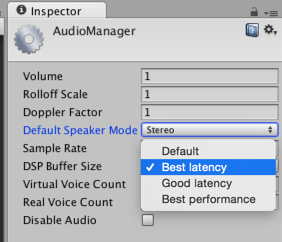
\includegraphics[scale=1]{./img/opti_sound.png}
  \caption{Paramètre pour la synchronisation des sons}
  \label{transitions_scenes}
\end{figure}

\subsection{Optimisation du poids de l'application}

Une application ne doit pas avoir un poids trop élevé si elle veut rester cohérente sur une vitrine.  Pour cela, Unity propose plusieurs façon de compresser les fichiers composant l'application. Ainsi, pour compresser les images utilisées dans les \textit{sprites}, il est possible de les compresser en diminuant leur taille initiale ou bien en choisissant un algorithme de compression différent.

Bien entendu cela impacte la qualité de jeu de l'utilisateur sur des périphériques à grand écran comme les tablettes ou les derniers smartphones, c'est pour cela que Unity propose de n'appliquer les compressions voulues seulement sur un déploiement en particulier. Par exemple, il est possible de compresser les textures sur les systèmes Android et iOS, mais de garder les textures en haute-définition pour un déploiement PC.


\begin{figure}[H]\centering
  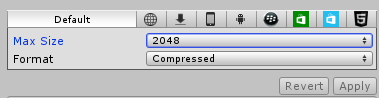
\includegraphics[scale=1]{./img/optimisation_poids.png}
  \caption{Aperçu des réglages de compression des textures}
  \label{optimisation_poids}
\end{figure}


